\documentclass[onecolumn, draftclsnofoot,10pt, compsoc]{IEEEtran}
\hbadness=1000 % suppress warnings
\usepackage{graphicx}
\usepackage{url}
\usepackage{setspace}
\usepackage{hyperref}
\usepackage{listings}
\usepackage{cite}
\usepackage{geometry}

\usepackage{longtable}

\geometry{textheight=9.5in, textwidth=7in}

% 1. Fill in these details
\def \CapstoneTeamName{		Aerolyzer}
\def \CapstoneTeamNumber{		19}
\def \GroupMemberOne{			Daniel Ross}
\def \GroupMemberTwo{			Logan Wingard}
\def \CapstoneProjectName{		Aerolyzer}
\def \CapstoneSponsorPerson{		Kim Whitehall}


% 2. Uncomment the appropriate line below so that the document type works
\def \DocType{		%Problem Statement
	%Requirements Document
	%Technology Review
	%Design Document
	Progress Report
}

\newcommand{\NameSigPair}[1]{\par
	\makebox[2.75in][r]{#1} \hfil 	\makebox[3.25in]{\makebox[2.25in]{\hrulefill} \hfill		\makebox[.75in]{\hrulefill}}
	\par\vspace{-12pt} \textit{\tiny\noindent
		\makebox[2.75in]{} \hfil		\makebox[3.25in]{\makebox[2.25in][r]{Signature} \hfill	\makebox[.75in][r]{Date}}}}
% 3. If the document is not to be signed, uncomment the RENEWcommand below
\renewcommand{\NameSigPair}[1]{#1}

%%%%%%%%%%%%%%%%%%%%%%%%%%%%%%%%%%%%%%%
\graphicspath{{images/}}
\begin{document}
	\begin{titlepage}
		\pagenumbering{gobble}
		\begin{singlespace}
			\centering
			
\includegraphics[height=4cm,natwidth=345,natheight=435]{images/coe_v_spot1.png}
			\hfill 
			% 4. If you have a logo, use this includegraphics command to put it on the coversheet.
			%\includegraphics[height=4cm]{CompanyLogo}   
			\par\vspace{.2in}
			\centering
			\scshape{
				\huge CS Capstone \DocType \par
				{\large\today}\par
				\vspace{.5in}
				\textbf{\Huge\CapstoneProjectName}\par
				\vfill
				{\large Prepared for}\par
				{\Large\NameSigPair{\CapstoneSponsorPerson}\par}
				{\large Prepared by }\par
				Group\CapstoneTeamNumber\par
				% 5. comment out the line below this one if you do not wish to name your team
				\CapstoneTeamName\par 
				\vspace{5pt}
				{\large
					\NameSigPair{\GroupMemberOne}\par
					\NameSigPair{\GroupMemberTwo}\par
				}
				\vspace{20pt}
			}
			\begin{abstract}  
				The Aerolyzer Project aims to deliver a new source of air quality and weather information through leveraging existing weather data and image analysis algorithms.
				When complete, this open-source project shall feature a Python library that uses image classification and third-party weather APIs, displayed with an intuitive web-based user interface.
				This document outlines the software design descriptions for the Aerolyzer Library. 
			\end{abstract}     
		\end{singlespace}
	\end{titlepage}

\tableofcontents
\clearpage

\begin{singlespace}

	\section{Project Purpose}
		Monitoring atmospheric aerosols is important due to their effects on people’s health and the atmosphere's chemical composition and radiation distribution.
		Currently delayed or inaccurate atmospheric reports complicate getting reliable local atmospheric information.
		Unfortunately, aerosols in the atmosphere are constantly changing, and current satellite, aircraft, and ground-based instruments do not simplify data enough for the average person to understand.
		There is currently no way to judge local air quality using regional aerosol data without in-depth atmospheric knowledge.
		Additionally, delayed or inaccurate atmospheric reports complicate getting reliable local atmospheric information.
		The primary objective of the Aerolyzer project is to create a tool that infers local air quality using regional weather data and image analysis.
		The major goals this presents to the project are a quick weather data retrieval, the identification of an image that can be used for color analysis, and the analysis of the colors in an image to estimate the level of aerosols.
	
	\section{Current State}
		
		\subsection{Logan Wingard}
			We have completed the entire Aerolyzer library and a more recent version has been uploaded to Pypi. 
			The app now calls the updated functions instead of not doing anything once the image is uploaded.
			The image restriction functions have been thouroughly tested for bugs and we are confident that these functions are working well enough for demonstrations.

			The poster went smoothly, and should be ready for pickup by now.
			We are pretty confident that our poster will make a great impression on the visitors of the expo and represent what Aerolyzer is about nicely.
			Here is the image that we used on our poster that will represent what our project does.
			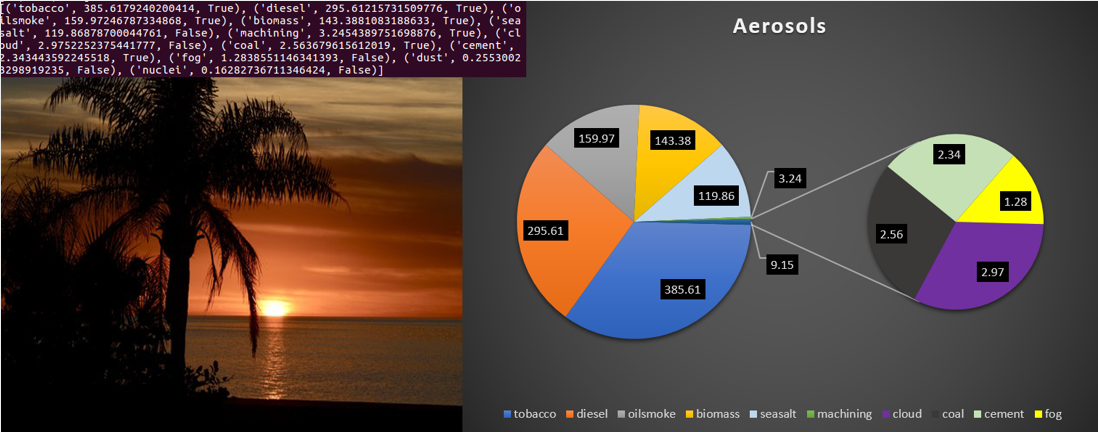
\includegraphics[height=4cm,natwidth=1098,natheight=432]{images/posterimg.png}
		\subsection{Daniel Ross}
			
			
			
	\section{What's left to accomplish}
		
		\subsection{Logan Wingard}
			The most recent version is not yet uploaded to Pypi, so that must be done before expo so that we can demo using the app and not running it from command line.
			There is quite a bit more implementation testing that we need to get done before expo as well.
			We need many valid images that meet all the requirements for demonstrations, and they not only need to be tested against our functions, but also through the app.
			We will soon need to submit all of our code that we have written over the course of the entire year, so we need to go through and write clear comments about what every line does to make it easier to grade/read.
			Lastly, we must present at expo.
			This is pretty intimidating, as there will be people of all levels of knowledge and possibly some employers looking for employees, though with some preparation, we will make a great face for Aerolyzer.
		\subsection{Daniel Ross}
			


	\section{Problems}
		
		\subsection{Logan Wingard}
			With such strict criteria of the image restriction functions, it is very difficult to find images that meet all of these criteria.
			There was also a large period of time when we were unable to contact out client Kim for a medical reason at the time unknown to us.
			We were eventually able to reconnect with Kim and get the project back on track so it is no longer an issue.
			There was an issue that our functions would call data from a config file that hadn't been made on the users computers, so my solution to this was to scrap the config files completely and instead make them variables in the classes.
			With this solution, we do not have to go through the hassle of making a function that writes the config file, though the drawback is our users will not be able to configure the image restriction criteria without digging into the code.
			The code is open source, so anyone who so chooses to alter the criteria is able to, though for less tech savvy users, it couold be intimidating. 
		\subsection{Daniel Ross}
			
			
	\section{Interesting Code}
		The following is an excerpt from the horizon detection function.
		It has since been updated with slightly different numbers in order to increase accuracy, but this is what is currently pushed to out master Aerolyzer github.
		It splits the image at the horizon and then splits the sky in half to analyze the histogram data in both the top and bottom half of the sky.
		These are used to further determine if the image is actually valid.
		If the image is valid, it moves onto color analysis with the bottom half of the sky.
		\begin{lstlisting}
color = ('b', 'g', 'r')
b, g, r = cv2.split(img)
dimy, dimx = img.shape[:2]

largest = [0, 0]
it = dimy / 200 #iterations = total number of rows(pixels) / 200
for i in range(dimy / 4, (dimy / 4) * 3, it):   #only looking at the middle half of the image
	ravg = (sum(r[i]) / float(len(r[i])))
	gavg = (sum(g[i]) / float(len(g[i])))
	bavg = (sum(b[i]) / float(len(b[i])))
	avg = (ravg + gavg + bavg) / 3
	pravg = (sum(r[i - it]) / float(len(r[i - it])))
	pgavg = (sum(g[i - it]) / float(len(g[i - it])))
	pbavg = (sum(b[i - it]) / float(len(b[i - it])))
	pavg = (pravg + pgavg + pbavg) / 3
	diff = pavg - avg
	if diff > largest[0]:   #only getting the largest intensity drop.
		largest = [diff,i-(it/2)]
if largest[0] >= 11:
	sky = img[0:largest[1],0:dimx]#cropping out landscape
	h1 = sky[0:(sky.shape[0] / 2),0:dimx]#top half of sky
	h2 = sky[(sky.shape[0] / 2):(sky.shape[0]), 0:dimx]#bottom half

	mask = np.zeros(h1.shape[:2], np.uint8)
	mask[0:(h1.shape[0] / 2), 0:h1.shape[1]] = 255

	for i,col in enumerate(color):
		histr = cv2.calcHist([h1], [i], mask, [255], [0, 255])
		plt.plot(histr, color = col)
		plt.xlim([0,255])

	mask = np.zeros(h2.shape[:2], np.uint8)
	mask[0:(h2.shape[0] / 2), 0:h2.shape[1]] = 255

	for i,col in enumerate(color):
		histr = cv2.calcHist([h2], [i], mask, [255], [0, 255])
		plt.plot(histr, color = col)
		plt.xlim([0, 255])
			\end{lstlisting}	
			Here are the results of this function:\\
			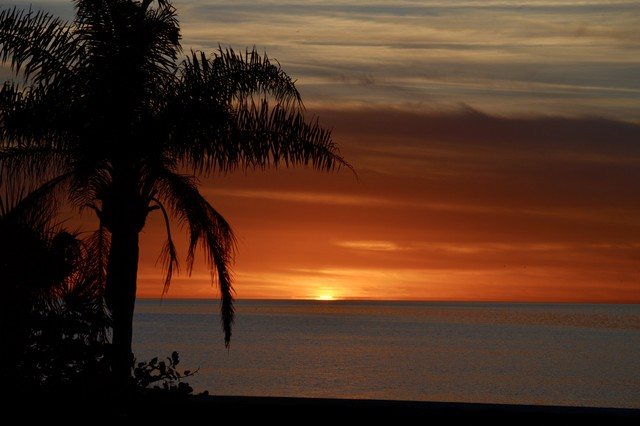
\includegraphics[height=4cm,natwidth=640,natheight=426]{images/horizon_uncropped.jpg}\\
			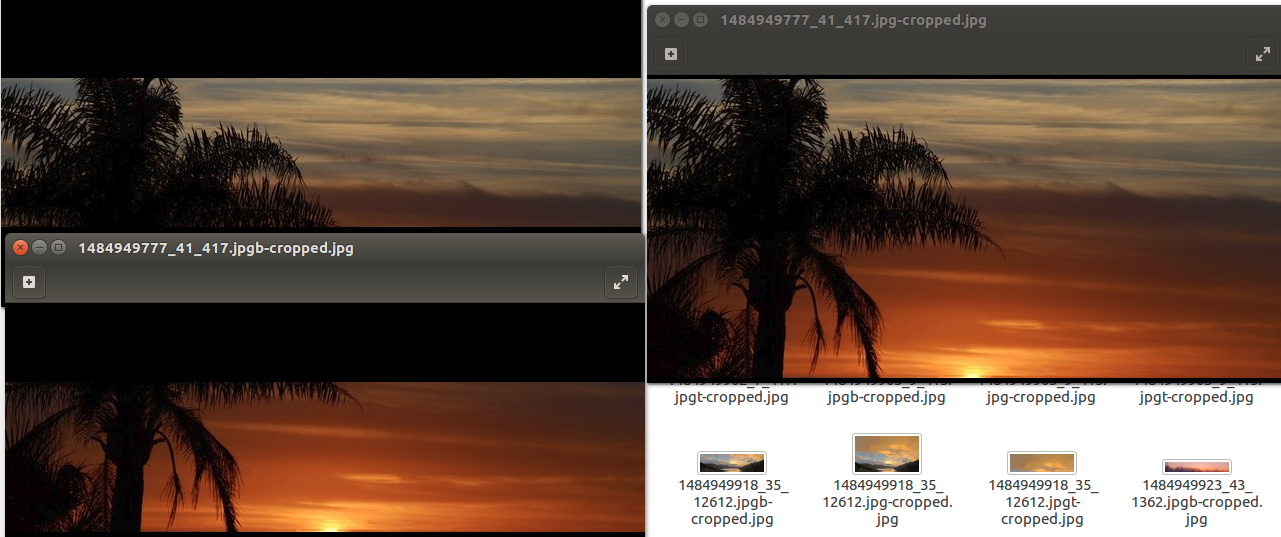
\includegraphics[height=4cm,natwidth=1281,natheight=537]{images/horizon_cropped.png}\\
			
			This code is my fix to the issue dealing with config files. 
			Instead of checking lists or values inside the list criteria, it checks vor values in types, devices, etc.
			This eliminates the need for config files entirely.
			\begin{lstlisting}
def __init__(self):
	self.types = [".png",".jpg",".jpeg",".JPG"]
	self.devices = ["iPhone 5","iPhone 5s","iPhone 6","iPhone 6s","DROIDX","SM-G730V","iPhone SE","SM-G920V"]
	self.maxSize = 4000000
	self.imgWidthMin = 100
	self.imgLengthMin = 100
	self.imgWidthMax = 6000
	self.imgLengthMax = 6000
	#self.criteria = self._import_yaml(os.getcwd() + "/../../Aerolyzer/aerolyzer/config/image_restriction_conf.yaml")
			\end{lstlisting}

			The following is the sun\_position function
			\begin{lstlisting}
def sun_position(exifdict):
	coord = get_coord(exifdict)
	wData = wunderData.get_data(str(coord[0])+","+str(coord[1]))
	sunriseTime = wData['sunrise'].split(':')
	sunsetTime = wData['sunset'].split(':')
	sunriseTarget = (int(sunriseTime[0])*60)+int(sunriseTime[1])
	sunsetTarget = (int(sunsetTime[0])*60)+int(sunsetTime[1])

	hoursTime = (str(exifdict['exif datetimeoriginal']).split(' '))[1].split(':')
	pictureTime = (int(hoursTime[0])*60)+int(hoursTime[1])+int(float(hoursTime[2])/60)

	if ((pictureTime >= (sunriseTarget - 15)) & (pictureTime <= (sunriseTarget + 30))):
		return 1
	elif ((pictureTime >= (sunsetTarget - 15)) & (pictureTime <= (sunsetTarget + 30))):
		return 2
	elif ((pictureTime > (sunsetTarget + 15))|(pictureTime < (sunriseTarget - 15))):
		return 0
	else:
		return 0
			\end{lstlisting}
\end{singlespace}
\clearpage
\bibliographystyle{IEEEtran}
\bibliography{ref}
\end{document}
